% 
% \newacronym{coo}{COO}{Chief Operating Officer}
% \newacronym{cto}{CTO}{Chief Technology Officer}
% \newacronym{cmo}{CMO}{Chief Marketing Officer}
% \newacronym{cio}{CIO}{Chief Information Officer}
% \newacronym{clo}{CLO}{Chief Legal Officer}
% \newacronym{cbdo}{CBDO}{Chief Business Development Officer}
% \newacronym{cro}{CRO}{Chief Risk Officer}
% \newacronym{cfo}{CFO}{Chief Financial Officer}
% \newacronym{cso}{CSO}{Chief Security Officer}
% \newacronym{cdo}{CDO}{Chief Data Officer}
% \newacronym{cco}{CCO}{Chief Communications Officer}
% 


\item Real-time database:


\item Cloud Messaging: allows developers to send push notification and targeted messages to a
client app that new email or other data is available to sync, or send notification messages to drive app
interaction, adding more user re-engagement and retention. It is a cross-platform messaging solution that lets
developers reliably deliver messages at no cost.
\item Remote Config: allows developers to dynamically control and the change behaviour and appearance of their apps
without publishing app updates and requiring users to download them.
\item Performance Monitoring
\item Analytics: provides free and unlimited analytics solutions for understanding app usage, user engagement and
user behaviour by tracking event logging, user demographics, and funnel analysis to gain valuable insights to
improve the app.
\item Crashlytics: is a lightweight, real-time crash and error reporter that helps developers track, prioritize,
and fix stability issues that erode to the quality of the developer's app.
\item Test Lab: enables automated testing of the developer's app on real devices in the Google data center.
\item Dynamic Links: consist of deep links that dynamically route users to the content they are interested in,
across platforms and devices. It helps developers create and share links that work the way they want, on the
platform they want, and whether users have their apps installed.
\item \acrshort{ml} Kit: provides a set of \acrshort{ml} \acrshort{api}s that can be easily integrated developer's app.
This feature is still in beta testing.


\textbf{JSON format}
\acrshort{json} is a lightweight data-interchange format that is easy for humans to read and write while being
also easy for machines to parse and generate too. It is based on a subset of the JavaScript programming language
and is commonly used for representing structured data. \acrshort{json} is often used for transmitting data between
a server and a web application, as well as for storing configuration data.

\acrshort{json} data is organized into key-value pairs, where keys are strings and value can be strings (enclosed
in double quotes `""`), booleans (`true` or `false`), numbers, objects (unordered collections of key-value pairs
enclosed in curly braces '{}'), arrays (ordered collections of values enclosed in square brackets '[]'), or null.
\end{multicols}

\begin{lstlisting}[language=JSON, caption=Example of a JSON response, label=lst:jsonresponse]
    {
          "name": "John Doe",
          "age": 30,
          "isStudent": false,
          "cars": [
                { "name": "Ford", "models": ["Fiesta", "Focus", "Mustang"] },
                { "name": "BMW", "models": ["320", "X3", "X5"] },
                { "name": "Fiat", "models": ["500", "Panda"] }
          ],
          "hobbies": ["Reading", "Gaming", "Traveling", "Cooking", "Photography", "Painting", "Gardening"],
          "address": {
                "street": "Sesame Main Street",
                "city": "New York",
                "zip": "10001"
          }
    }
\end{lstlisting}

\begin{multicols}{2}
      \textbf{XML format}

      \acrshort{xml} is a markup language that defines a set of rules for encoding documents in a format that
      is both human and machine-readable. It provides a way to structure data in a hierarchical format using
      tags to define elements and attributes within those elements. It is often used for storing, designing, and
      representing structured data in a portable and platform-independent way, making it easy to create,
      exchange, and process information between different systems, applications, and platforms.

      \acrshort{xml} documents consist of text-based data enclosed in tags, like \acrshort{html}, but
      allows users to define their own customized tags and document structures. This flexibility makes
      \acrshort{xml} suitable for representing a wide variety of data types and structures.

      \acrshort{xml} is often used in various domains such as web services, configuration files, data
      interchange between different software systems, and more.
\end{multicols}

\begin{lstlisting}[language=XML, caption=Example of a XML response, label=lst:xmlresponse]
    <?xml version="1.0" encoding="UTF-8"?>
    <response>
        <status>200</status>
        <message>OK</message>
        <data>
            <user>
                <id>123</id>
                <username>johndoe</username>
                <email>johndoe@example.com</email>
                <role>user</role>
            </user>
            <user>
                <id>456</id>
                <username>janedoe</username>
                <role>admin</role>
            </user>
        </data>
    </response>
\end{lstlisting}

\textbf{OpenAPI Standard}

Previously known as Swagger, \acrshort{oas} is a specification for writing a public \acrshort{api}, with
guidelines for details like endpoint naming conventions, data formats, and error messaging
(\cite{openapistandard}). The standards required by Open\acrshort{api} and its automation of some tasks
make it easier for a developer to start working with an \acrshort{api} without needing to read through
a complex code base. For \acrshort{api} producers, Open\acrshort{api} standard offers access to a wide
variety of tools based on the standards. \acrshort{api} teams can use these tools to quickly up mock
servers and create high-quality documentation, among other tasks.
\acrshort{api}s are generally categorized into different types based on their audience, architecture, and
protocols (\cite{typesofapi}):

\begin{multicols}{2}


      \subsubsection{Flutter}
      Flutter is an open-source framework made by Google in 2017. It used as an \acrshort{ui} toolkit for building
      natively compiled applications for mobile, web, and desktop (Windows, mac\acrshort{os}, Linux) from a single
      codebase (\textit{\cite{flutter}}).

      \textbf{Widgets}

      Widgets in Flutter refer to the basic building blocks used to build \acrshort{ui}s. Everything in Flutter, from
      buttons to layout containers to text inputs, is a widget. They are lightweight, reusable components that
      define the structure, appearance, and behavior of \acrshort{ui} elements in a Flutter application. When a widget's
      state changes, the widget rebuilds its description, which the framework diffs against the previous description
      to determine the minimal changes for rendering in the \acrshort{ui}. There are only 2 types of Widgets
      in Flutter:
      \begin{itemize}
            \item \textbf{Stateless Widget}: is immutable, meaning that their properties cannot change once they are
                  initialized. They are used for static content that does not require user interaction. Examples of a
                  stateless widget would be text labels, buttons, icons, and static images.
            \item \textbf{Stateful Widget}: it maintains state, allowing their properties to change over time in response
                  to user interactions or other events. They are used for dynamic content that require updates, such as
                  animations, form inputs, and interactive elements. Stateful widgets consist of two classes: the widget
                  class itself and a corresponding state class that manages the widget's state. Examples of stateful widgets
                  are: text input fields, scrollable lists, tabs, and progress indicators.
      \end{itemize}
      Flutter apps are built using a hierarchy of nested widgets, forming a "widget tree". The root widget defines the
      overall app structure, and other widgets branch out to create more complex \acrshort{ui}s.
\end{multicols}

\begin{lstlisting}[language=Dart, caption=Example of a stateful and stateless widget, label=lst:dartWidgets]
// Stateless Widget
class MyTextWidget extends StatelessWidget {
      final String text;

      MyTextWidget({Key key, this.text}) : super(key: key);

      @override
      Widget build(BuildContext context) {
      return Text(text);
      }
}

// Stateful Widget
class MyCheckbox extends StatefulWidget {
      @override
      _MyCheckboxState createState() => _MyCheckboxState();
}

class _MyCheckboxState extends State<MyCheckbox> {
      bool isChecked = false;

      @override
      Widget build(BuildContext context) {
            return Checkbox(
                  value: isChecked,
                  onChanged: (bool value) {
                        setState(() {
                        isChecked = value;
                  });
            });
}
}
\end{lstlisting}

\begin{multicols}{2}


      \textbf{NoSQL Database}

      is a category of \acrshort{db} that provides a mechanism for storage and retrieval of data that is modelled in ways other
      than the tabular relations used in \acrshort{rdbms}. \acrshort{nosql} \acrshort{db}s are typically designed to handle large
      volumes of unstructured or semi-structured data, such as \acrshort{json}, \acrshort{xml}, or binary objects, and they offer
      a flexible data model that can evolve over time. Both databases in Firebase, Firestore, and Real-time Database are \acrshort{nosql}
      databases. Some characteristics of \acrshort{nosql} \acrshort{db}s include (\cite{nosql}):
      \begin{itemize}
            \item Data Model: \acrshort{nosql} uses dynamic schema, which allows data to be inserted without having to define the schema
                  first, while \acrshort{sql} uses a fixed schema to store data.
            \item Data Structure: \acrshort{nosql} \acrshort{db}s use a variety of data structures such as key-value pairs,
                  document-oriented, graphs databases, and columns-oriented; unlike \acrshort{sql} which only uses tables to store data.
            \item Querying: \acrshort{nosql} uses variety of query languages, such as Mongo\acrshort{db} query language or Cassandra's
                  \acrshort{cql}, while \acrshort{sql} databases only use \acrshort{sql} as the unified language to query data.
            \item Data Consistency and \acrshort{acid} Compliance: databases that are \acrshort{acid} compliant means that they follow a
                  set of rules to ensure that database transactions are processed reliably and securely. \acrshort{sql} databases are a
                  good example of this, while \acrshort{nosql} databases sacrifice some \acrshort{acid} properties to achieve higher
                  performance and scalability.
            \item Use Case: \acrshort{nosql} \acrshort{db}s are ideal for applications that need to handle large volumes of data and
                  require high scalability and flexibility, such as social media platforms, real-time analytics, and content management
                  systems.
            \item Scalability: \acrshort{nosql} databases are traditionally designed for horizontal scalability, meaning they can easily
                  scale out multiple servers or clusters to handle volumes of data and high throughput, which is more cost-effective and
                  allows for better scalability. They are well-suited for distributed and cloud-based environments. \acrshort{sql}
                  databases are traditionally designed for vertical scalability, meaning a single server is scaled up with more powerful
                  hardware and power (\acrshort{cpu}, \acrshort{ram}) to a single server. This can become expensive and limit scalability.
      \end{itemize}
\end{multicols}

\begin{figure}[htbp]
      \centering
      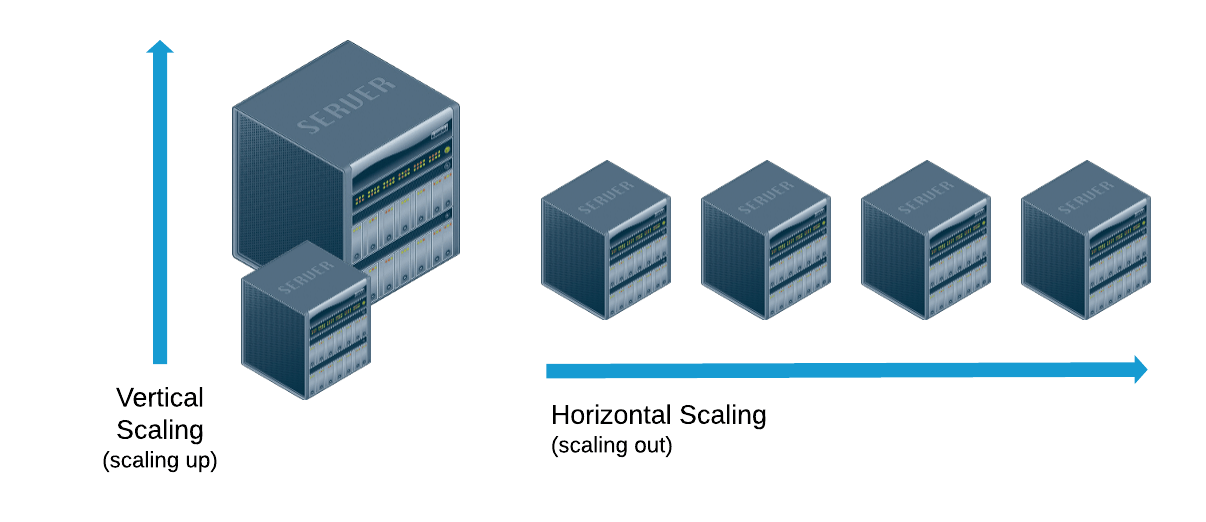
\includegraphics[width=0.8\textwidth]{Figures/nosql-scalling.png}
      \caption{Vertical (\acrshort{sql}) \acrshort{vs} Horizontal (\acrshort{nosql}) Scaling}
      \label{fig:graphqlvsrestarchitecture}
\end{figure}

\begin{multicols}{2}
      Some examples of \acrshort{nosql} databases include Mongo\acrshort{db} (document-oriented), Cassandra (wide-column store), Redis
      (key-value store), and Neo4j (graph database). Some examples of \acrshort{sql} databases include My\acrshort{sql},
      Postgres\acrshort{ql}, and \acrshort{ms} \acrshort{sql} Server.
      \subsection{Q-ICT Internal APIs}
      \subsubsection{What is an API?}
      \acrshort{api} is a software intermediary that allows two applications to talk to each other. They are an
      accessible way to extract and share data within and across organizations.
      \subsubsection{Web APIs}
      A web \acrshort{api} is an \acrshort{api} that can be accessed using the \acrshort{http} protocol. Not all
      \acrshort{api}s are web \acrshort{api}s; some \acrshort{api}s are used only to communicate between two
      applications on the same computer, never making use of a web connection. But in practice, when developers talk
      about \acrshort{api}s, they are almost always talking about web-based \acrshort{api}s used to


      \item Real-time database: is also a cloud-hosted \acrshort{nosql} \acrshort{db} that lets the user store
      and sync data between users in real-time (\textit{\cite{realtimeDatabase}}).

      \textbf{JavaScript}

      \acrshort{js} is a high-level, interpreted programming language that conforms to the \acrshort{ecma}Script specification.
      It is a multi-paradigm programming language, supporting \acrshort{oop}, imperative, and functional programming styles and
      is primarily used for client-side web development. It is also used for server-side development with Node.js, and for
      mobile app development with frameworks like React Native, Vue.js, Angular.js, and NativeScript. \acrshort{js} is now one
      of the core technologies of the web, along with \acrshort{html} and \acrshort{css}, and is supported by all modern web
      browsers. Some key features of \acrshort{js} include:
      \begin{itemize}
            \item Client-side Scripting: it is mainly used for client-side scripting in web browsers, allowing programmers to
                  create dynamic content that interacts with the browser and the user. It can manipulate the content and behavior
                  of \acrshort{html} elements, respond to user actions without the need to reload the page for interacting with
                  \acrshort{dom} to update page content dynamically. This enhances the \acrshort{ux} by making web applications
                  feel more responsive and integrated.
            \item Cross-Platform Compactibility: it is supported by all modern web browsers, including Chrome, Firefox, Safari,
                  Opera, and Edge, and can be used to build cross-platform web applications that run on any device or platform,
                  like Android or i\acrshort{os}.
            \item Server-Side Scripting: with the advent of Node.js, it has also become popular for server-side scripting. Node.js
                  is a runtime environment that allows developers to build scalable network applications, including web servers,
                  \acrshort{api}s, and real-time applications like chat servers. This has expanded the versatility and use cases of
                  \acrshort{js} beyond the browsers, making it a full-stack development language.
            \item Dynamic Typing: it means that variables do not have predetermined types. Instead, types are determined at runtime
                  based on the assigned values.
            \item Functional Programming: it supports concepts such as first-class functions, high-order functions, and closures.
                  This allows programmers to write more concise and expressive code by treating functions as first-class citizens.
            \item Event-Driven Programming: it follows an event-driven programming paradigm, where actions or events trigger specific
                  functions or code execution, makes it well-suited for building interactive \acrshort{ui} and handling user interaction.
      \end{itemize}
      \textbf{Node.js}

      is an open-source, cross-platform, server-side runtime environment built on Chrome's V8 \acrshort{js} engine that allows
      programmers to run \acrshort{js} code outside a web browser, enabling the development of server-side and networking applications.

      \textbf{TypeScript}

      is an open-source programming language developed and maintained by Microsoft. It is a superset of \acrshort{js}, meaning that any valid
      \acrshort{js} code is also valid in \acrshort{ts}. It adds optional static typing to \acrshort{js}, which allows developers to
      annotate their code with type information, catch errors early in the development, and improve the maintainability or large codebases. Some
      developers prefer using \acrshort{ts} over \acrshort{js} for some of its key-features:
      \begin{itemize}
            \item Static Typing: it checks the types of variables at compile-time, which enable developers to specify the types of
                  variables, functions parameters, and return values. This introduces type safety, in contrast to \acrshort{js} which is
                  dynamically typed, which means that the types of variables are determined at runtime.
            \item Enums: it provides support for enums, allowing developers to define a set of named constants with associated values.
            \item Generics: it supports generics, enabling the creation of reusable components that can work with a variety of data types.
            \item Decorators: it supports decorators, which are a way to add annotations and a meta-programming syntax for class
                  declarations and  members. Decorators can be used to modify classes, methods, and properties at design time, providing a
                  powerful way to extend or modify the behaviour of classes and their members.
            \item Interfaces and Classes: it supports \acrshort{oop} concepts such as classes, interfaces, inheritance, and access modifiers,
                  making it easier to organize and structure code.
            \item \acrshort{es}6+ Features: it supports many features introduced in \acrshort{ecma}Script standards beyond \acrshort{es}5,
                  such as arrow functions, classes, async/await syntax, and modules.
            \item Backwards Compactibility: it is designed to be backwards compactible with \acrshort{js}, which means that developers can
                  use it alongside \acrshort{js} code and integrate it into existing \acrshort{js} projects and environments, including,
                  browsers, Node.js, and other \acrshort{js} runtime environments.
      \end{itemize}
\end{multicols}

\begin{figure}[htbp]
      \centering
      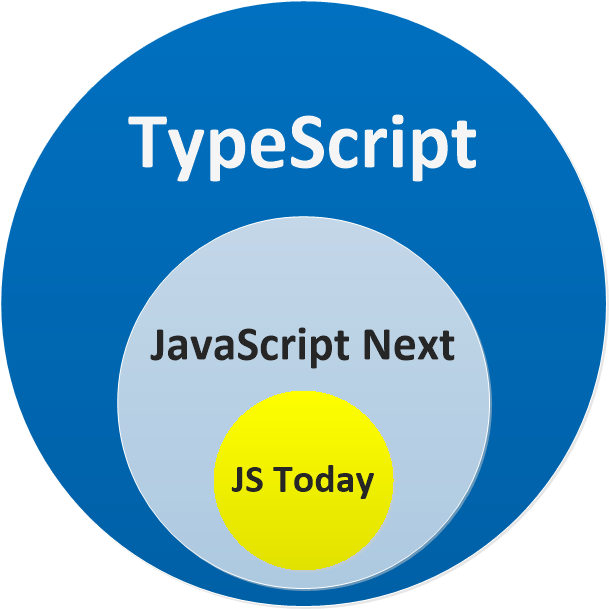
\includegraphics[width=0.6\textwidth]{Figures/TSJSVenn.png}
      \caption{Venn diagram of TypeScript and JavaScript}
      \label{fig:tsjsvenn}
\end{figure}

\begin{multicols}{2}


\textbf{Composite API}: it connects multiple \acrshort{api}s into a single data or interface or process to
streamline the development operations, therefore allowing developers to bundle and send requests from different
\acrshort{api}s as they do not have to write separate code for every individual \acrshort{api}. Usually,
one or more related \acrshort{api}s are combined to improve performance. They reduce the load to the server
as they are treated as a single call. In the microservice-based architecture
(\textit{\nameref{microservicesapi}}), a single user action might involve multiple calls, which can come as
a drawback as they generate enormous number of individual \acrshort{api} calls. In that scenario, the orchestration
of this type of \acrshort{api} is very helpful as this work faster and is easier to implement. It is more secure
than using multiple, individualized solutions, and it may also support multiple \acrshort{api} protocol types.

A good example of this type is Shopify \acrshort{api}, which provides synchronization to large volumes of data and
actions with other platforms that are dependent on each other in one request, such as Etsy, eBay, and Amazon. Rather
than having multiple \acrshort{api}s to manage the automation of inventory, shipping, and taxes across multiple shopfronts,
a single \acrshort{api} can be used for syncing and integration. Similar in ordering via a food app, the customers can
use multiple GET calls, retrieving the food, and finally placing the request as a POST call.
\subsubsection{Different Types of API by Architecture}
\textbf{Monolithic API}: this is a single, coherent codebase type of architecture, providing access to a complex data
source. Most public \acrshort{api}s are monolithic \acrshort{api}s, because it is familiar to most web developers, and
they often closely follow the \acrshort{mvc} architecture of a relational \acrshort{db}. They provide predictable
functionality across a range of resources, and they generally remain fairly stable over time because they serve so
many use cases for many users.

However, as the name suggests, they are monolithic, and therefore can be difficult to scale or refactor, because so much
data is interconnected with them. When developers worry about releasing "breaking changes", they are often working with
monolithic architectures, where changing even minor details can have unpredictable consequences.

\textbf{Microservices API} \label{microservicesapi}: this is the main alternative to monolithic \acrshort{api}
architecture. This architecture is more common for internal and partner \acrshort{api}, though public \acrshort{api}
may also be part of an organization's overall microservice architecture. Most development teams using a
\acrshort{ci}/\acrshort{cd} process make use of many microservices as part of their code lifecycle, each serving a
discrete, independent purpose. For example, an e-commerce company might have an internal microservice that
provides inventory data, and another to validate employee geolocation on changes to inventory data, while
software developers pushing code automatically call microservices for testing and governance. As workflows
change, individual microservices can be swapped out, updated, or replaced without affecting the overall parts
of the system.

\textbf{Unified API}: this type is common among Partner \acrshort{api}s. It serves similar purpose to Composite
\acrshort{api}s, but instead it bundles related calls to multiple different \acrshort{api}s, instead of to multiple
endpoints on a single \acrshort{api}.

\begin{longtable}{|p{8cm}||p{8cm}|}
      \hline
      \rowcolor{blue!20}
      \acrshort{rest}                                                            & \acrshort{soap}                              \\
      \endfirsthead
      \hline
      Works with \acrshort{xml}, \acrshort{json}, \acrshort{http} and plain text & Works with \acrshort{xml} by design          \\
      \hline
      Loose and flexible guidelines based on architectures                       & Strict, clearly-defined rules                \\
      \hline
      Modest security                                                            & Advanced security                            \\
      \hline
      Works well with data                                                       & Works well with processes (actions)          \\
      \hline
      Uses low bandwidth and is highly scalable                                  & Uses more bandwidth with limited scalability \\
      \hline
      \caption{Comparison of REST and SOAP}
      \label{tab:restvsoap}
\end{longtable}

\begin{multicols}{2}
      \textbf{GraphQL API}:
      is contract-driven and come with introspection out-of-the-box. It was developed by Facebook for internal purposes
      in 2012, and it was open-sourced in 2015. Now it is maintained by the Graph\acrshort{ql} Foundation (\cite{graphql}).
      Building an \acrshort{api} with Graph\acrshort{ql} is very easy in comparison to true \acrshort{rest} \acrshort{api}s,
      which require extensive knowledge of \acrshort{http} to build intelligently.

      The downside is, however, that they do not scale well and require tight coupling between the client and the
      server. Graph\acrshort{ql} queries get more expensive to parse and execute plans for as they get bigger and
      lack certain concepts native to \acrshort{http}, such as content and language negotiation.
\end{multicols}
\begin{lstlisting}[language=JavaScript, caption=GraphQL's Schema Example]
      type Query {
            user(id: ID!): User
            posts: [Post!]!
      }
      type User {
            id: ID!
            name: String
      }
      type Post {
            id: ID!
            title: String!
            body: String!
      }
\end{lstlisting}
\begin{lstlisting}[language=JavaScript, caption=GraphQL's Request Example to Specific Data]
      {
            posts {
                  title
                  user(id: "123") {
                        name
                  }
            }
      }
\end{lstlisting}
\begin{lstlisting}[language=JavaScript, caption=GraphQL's Return Data Example]
{
      "data": {
            "posts": [
                        {
                              "title": "My first post",
                                    "user": {
                                          "name": "John Doe"
                                    }
                        }
                  ]
      }
}            
\end{lstlisting}
\begin{figure}[htbp] % here, top, bottom, page of floats
      \centering
      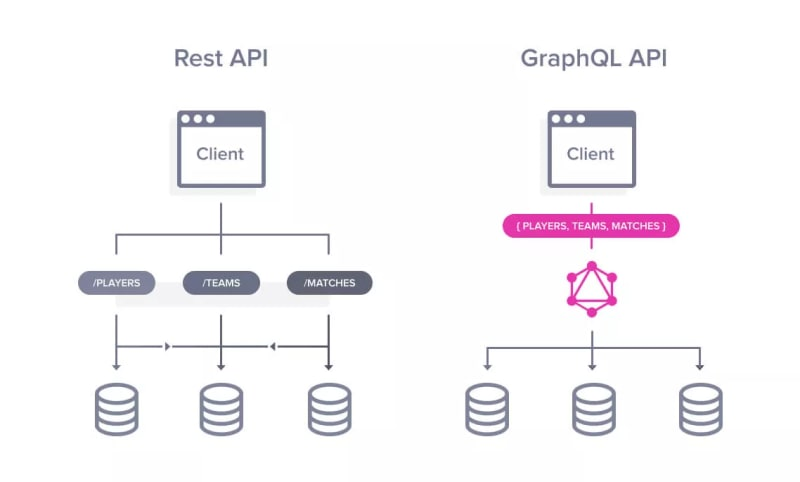
\includegraphics[width=0.8\textwidth]{Figures/graphql.jpg}
      \caption{GraphQL vs. REST Architecture}
      \label{fig:graphqlvsrestarchitecture}
\end{figure}
\begin{multicols}{2} % (json-rpc, xml-rpc, grpc) Webhooks API, Socket API Database API, Third-party API, Apache Thrift API, MsgPack API, SSE API, 
      \textbf{RPC API} : \acrshort{rpc} is a protocol return \acrshort{xml} or \acrshort{json} response. This protocol
      calls a method rather than a data resource, and remains one of the oldest and most stable protocols for
      \acrshort{api}s. While \acrshort{rest}ful \acrshort{api} returns a document, the response from a \acrshort{rpc}
      server is a confirmation that the function was triggered, or an error indicating  why it failed to run.

      \acrshort{rpc} is much faster than \acrshort{rest}, but the specifics depend on implementation. Unlike
      \acrshort{rest} or \acrshort{soap}, the message format varies. \acrshort{rpc} is tailored toward a client-server
      architecture and generally over a network.

      Components of a \acrshort{rpc} system:
      \begin{itemize}[label=$\star$]
            \item Client: the requesting device.
            \item Client stub: how the client will pack/unpack its materials.
            \item \acrshort{rpc} runtime: the messaging system (a courier between the client and server).
            \item Server stub: how the server will pack/unpack its materials.
            \item Server: the supplying device.
      \end{itemize}

      The popular frameworks of \acrshort{rpc}s are Apache Thrift, \acrshort{grpc}, and \acrshort{json}-\acrshort{rpc},
      and \acrshort{xml}-\acrshort{rpc}.

      \textit{gRPC}: developed by Google and released to public in 2015 to use, \acrshort{grpc} is an open-source
      \acrshort{rpc} architecture that can operate in numerous environments.

      The \acrshort{grpc} transport layer primarily relies on \acrshort{http}. The ability for developers to specify
      custom functions that allow for flexible inter-service communication is a significant feature of \acrshort{grpc}.
      This \acrshort{api} protocol also offers extra features such as timeouts, authentication, and flow control.

      In the \acrshort{grpc} protocol, data is transmitted in protocol buffers, a platform and language-agnostic mechanism
      that allows for data to be structured intuitively. This mechanism defines the service and then the data structures
      that the service will use. Compiling is taken care by protoc, the protocol buffer compiler.

      The output of this process is a comprehensive class containing the user's defined data types and basic set of methods
      in the chosen development language. Users can implement in-depth \acrshort{api} operations using this class.
\end{multicols}

\begin{lstlisting}[caption=gRPC Service For a Calculator In a Protobuf File]
      syntax = "proto3";

      package calculator;

      service Calculator {
            rpc Add(AddRequest) returns (AddResponse);
            rpc Subtract(SubtractRequest) returns (SubtractResponse);
      }

      message AddRequest {
            int32 a = 1;
            int32 b = 2;
      }

      message AddResponse {
            int32 result = 1;
      }

      message SubtractRequest {
            int32 a = 1;
            int32 b = 2;
      }

      message SubtractResponse {
            int32 result = 1;
      }
\end{lstlisting}

\begin{multicols}{2}
      \textit{Apache Thrift}: developed by Facebook, Thrift itself is a lightweight, language-agnostic software stack.
      This \acrshort{api} protocol supports \acrshort{http} transmission, along with binary transport formats. Thrift
      is capable of clean abstraction and implementations for data serialization and transport and application-level
      processing. Its primary objective is point-to-point \acrshort{rpc} implementation.

      Apache can support 28 programming languages, allowing programs written in any of these languages to communicate
      with each other and request remote services using \acrshort{api}s.
      \textbf{WebSocket}:
\end{multicols}

\begin{lstlisting}[language=JavaScript, caption=WebSocket's Example]
      // Client-side code
      const socket = new WebSocket('wss://example.com/socket'); // Replace with actual server's websocket URL
      
      // Event handler for when the connection is established
      socket.addEventListener("open", (event) => {
            console.log('Connected to the server');
            // Send data to the server
            socket.send('Hello, server!');
      });

      // Event handler for incoming messages from the server
      socket.addEventListener("message", (event) => {
            console.log(`Message from server: ${event.data}`);	
      });

      // Event handler for when the connection is closed
      socket.addEventListener("close", (event) => {
            console.log('Connection to the server closed');
      });

      // Event hander for handling errors
      socket.addEventListener("error", (event) => {
            console.error(`An error occurred: ${event.message}`);
      });
\end{lstlisting}

\begin{multicols}{2}
      \textbf{Socket}: is a software abstraction that allows programs running on different devices to
      communicate with each other over a network. It provides a standard interface for network
      communication, enabling data to be sent and received between applications running on separate
      computers. Sockets are commonly used in networking applications to establish connections and
      exchange data.
\end{multicols}

\begin{lstlisting}[language=Python, caption=TCP Server Example Using Sockets in Python]
      import socket

      # Create a TCP/IP socket
      server_socket = socket.socket(socket.AF_INET, socket.SOCK_STREAM)

      # Bind the socket to the address and port
      server_address = ('localhost', 8080)
      server_socket.bind(server_address)

      # Listen for incoming connections (max 5 clients in the queue)
      server_socket.listen(5)

      print('Server is listening on port 8080 for incoming connections....')

      while True:
            # Wait for a connection
            client_socket, client_address = server_socket.accept()

            try:
                  # Receive data from the client
                  data = client_socket.recv(1024)
                  print(f"Received data from {client_address}: {data.decode('utf-8')}")

                  # Send a response back to the client
                  response = 'Hello, client!'
                  client_socket.sendall(response.encode('utf-8'))

            finally:
                  # Clean up and close the connection
                  client_socket.close()
\end{lstlisting}

%       Additionally, threats can also be filtered from:
% \end{multicols}
% \begin{longtable}{|p{4cm}|p{4cm}|p{4cm}|p{4cm}|}
%       \hline
%       \rowcolor{blue!20}
%       Analysis Verdict (performed by user, marking it as) & Threat Mitigation Status & Incident Status & \acrshort{ai} Confidence level \\
%       \endfirsthead
%       \hline
%       \begin{itemize}
%             \item False positive
%             \item Suspicious
%             \item True positive
%             \item Undefined
%       \end{itemize}                                &
%       \begin{itemize}
%             \item Mitigated
%             \item Not mitigated
%             \item Marked as benign
%       \end{itemize}                              &
%       \begin{itemize}
%             \item Resolved
%             \item Unresolved
%             \item In progress
%       \end{itemize}                                   &
%       \begin{itemize}
%             \item Malicious
%             \item Suspicious
%             \item \acrshort{na}
%       \end{itemize}                                                                                                                \\
%       \hline
%       \caption{Different filters that can be applied to the Incidents page \#1}
% \end{longtable}
% \begin{longtable}{|p{4cm}|p{4cm}|p{4cm}|p{4cm}|}
%       \hline
%       \rowcolor{blue!20}
%       Engine                                           & Cloud Provider & \acrshort{os} & Classification \\
%       \endfirsthead
%       \hline
%       \begin{itemize}
%             \item SentinelOne Cloud
%             \item On-Write Static \acrshort{ai} - Suspicious
%             \item Behavioral \acrshort{ai}
%             \item On-Write Static \acrshort{ai}
%             \item Reputation
%             \item Cloud Detection
%             \item User-Defined Blocklist
%             \item Documents, Scripts
%             \item Anti Exploitation / Fileless
%             \item Intrusion Detection
%             \item Potentially unwanted application
%             \item Lateral Movement
%             \item Remote Shell
%             \item Manual
%             \item Application Control
%             \item Threat Intelligence
%             \item \gls{watchtower}
%             \item Driver Blocking
%       \end{itemize} &
%       \begin{itemize}
%             \item Azure
%             \item \acrshort{aws}
%             \item \acrshort{gcp}
%             \item \acrshort{oci}
%             \item ESXi
%       \end{itemize}                             &
%       \begin{itemize}
%             \item Windows
%             \item Linux
%             \item Mac
%             \item Windows Legacy
%       \end{itemize}                             &
%       \begin{itemize}
%             \item Malware
%             \item \acrshort{pua}
%             \item Virus
%             \item Infostealer
%             \item Hacktool
%       \end{itemize}                                                                                \\
%       \hline
%       \caption{Different filters that can be applied to the Incidents page \#2}
% \end{longtable}
% \begin{longtable}{|p{4cm}|p{4cm}|p{8cm}|}
%       \hline
%       \rowcolor{blue!20}
%       Initiated by                            & Time & Free text search                                                                                                                \\
%       \endfirsthead
%       \hline
%       \begin{itemize}
%             \item Agent Policy
%             \item Full Disk Scan
%             \item Local agent command
%             \item Deep Visibility Command
%             \item Management console \acrshort{api}
%             \item On-Demand Scan
%             \item Custom Rule
%             \item Custom Alert
%             \item Cloud Detection
%             \item Threat Intelligence
%             \item \gls{watchtower}
%       \end{itemize} &
%       \begin{itemize}
%             \item Recent
%             \item Last 24 Hours
%             \item Today
%             \item Last 48 Hours
%             \item Last 7 Days
%             \item Last 30 Days
%             \item This Month
%             \item Last 2 Month
%             \item Last 3 Month
%             \item Last Year
%             \item Custom Range
%       \end{itemize}                     &
%       \begin{itemize}
%             \item Content Hash
%             \item Cloud Account
%             \item Cloud Image
%             \item Cloud Instance \acrshort{id}
%             \item  Cloud Instance Size
%             \item Cloud Location
%             \item Cloud Network
%             \item   \acrshort{aws} Role
%             \item   \acrshort{aws} Security Groups
%             \item   \acrshort{aws} Subnet \acrshort{id}s
%             \item  Azure Resource Group
%             \item \acrshort{gcp} Service Account
%             \item Threat Details: \acrshort{eg} "This is a non-Microsoft binary that masquerades as a Microsoft executable"
%             \item File Path: \acrshort{eg}: "\textbackslash Device\textbackslash HarddiskVolumeA\textbackslash Users\textbackslash Chris\textbackslash Downloads\textbackslash malicious.exe"
%             \item Endpoint Name: \acrshort{eg} "LT-Christopher", "LT 10-08"
%             \item \gls{UUID}: \acrshort{eg}: "0ff2a3409f284776a23432e9f6894afa"
%             \item Agent Version (at detection) \acrshort{eg}: "23.1.4.650"
%             \item Agent Version (current)
%             \item Domain (at detection time)
%             \item Command Line Arguments
%             \item Initiated By (username): \acrshort{eg} "LuukAdmiraalMKBIT"
%             \item Storyline
%             \item Originated Process
%             \item Cluster Name
%             \item Node Name
%             \item Namespace Name
%             \item Namespace Labels
%             \item Controller Name
%             \item Controller Labels
%             \item Pod Name
%             \item Pod Labels
%             \item Container Name
%             \item Image Name
%             \item Container Labels
%             \item External Ticket \acrshort{id}
%             \item Node Labels
%       \end{itemize} \\
%       \hline
%       \caption{Different filters that can be applied to the Incidents page \#3}
% \end{longtable}

% \begin{multicols}{2}
Furthermore, it will also analyze for infected endpoint connectivity (offline/online), mitigated preemptively (yes/no),
reboot required (yes/no), action failed (yes/no), pending actions (yes/no), and if note and external ticket exists (yes/no).

\begin{multicols}{2}
      \textbf{MsgPack}: is an open standard for compact binary data serialization, ideal for efficient data transfer.
      \acrshort{msgpack} supports a variety of data types, including integers, floating-point numbers, strings,
      arrays, maps (key-value pairs), and more. It is designed to be platform-agnostic, meaning that the data can be
      serialized in one programming language and deserialize it in another without compactibility issues.
\end{multicols}

\begin{lstlisting}[language=Python, caption=MsgPack Serialization and Deserialization in Python]
      import msgpack

      # Creating a Python dictionary to represent some data
      data = {
            'name': 'John Doe',
            'age': 30,
            'is_student': False,
            'hobbies': ['Reading', 'Gaming', 'Traveling'],
            'address': {
                  'street': 'Sesame Main Street',
                  'city': 'New York',
                  'zip': '10001'
            }
            "scores": [90, 85, 95, 100, 95, 88, 72]
      }

      # Serialize the data to a MsgPack binary format
      packed_data = msgpack.packb(data)

      # Deserialize the MsgPack binary data back to a Python object
      unpacked_data = msgpack.unpackb(packed_data)

      # Print the original data and the deserialized data
      print("Original data:", data)
      print("Unpacked data:", unpacked_data)
\end{lstlisting}


\subsection{What is API Monitoring?}
\acrshort{api} monitoring is the process of gathering, visualizing, tracking, analyzing, and alerting on the
performance, availability, and the \acrshort{api} telemetry data to ensure that \acrshort{api} requests are
handled as expected.
\subsection{How Does API Monitoring Work?}
\acrshort{api} monitoring automatically checks \acrshort{api} performance and availability at regular intervals,
to ensure that the \acrshort{api} runs appropriately. This can be done in a few different ways, depending on the
type of the \acrshort{api} being monitored~\ref{chap:typesofapis}.

For example, let's take Postman, a popular free \acrshort{api} monitoring tools that allows developers to easily
monitor, analyze, and debug their \acrshort{api}s. In this example, the system might look for common errors, such
as 500-level responses or timeouts, when making requests to the \acrshort{api}. It also checks for latency issues
or sudden spikes in traffic that could indicate potential system problems. In addition, this monitoring system can
be configured to track specific metrics such as total requests, response times, and other \acrshort{kpi}s over time.
This will then provide real-time insights into \acrshort{api} performance and offers a range of features such as
automated alerts, detailed analytics, and comprehensive reporting capabilities. Features that an \acrshort{api}
monitoring might have are listed in the following (\cite{postmanapimonitoring}):
\begin{itemize}
      \item \textbf{Endpoint Surveillance}: it begins by closely tracking the various endpoints of an \acrshort{api}
            system. These endpoints represent specific functionalities or resources that the \acrshort{api} provides.
      \item \textbf{Request-Response Analysis}: monitoring tools can simulate \acrshort{api} requests by sending
            predefined inputs and parameters to specific endpoints, then analyzing the responses for relevant factors
            such as response time or data accuracy.
      \item \textbf{Performance Metrics Measurement}: \acrshort{kpi}s, such as response time, latency, and error rates,
            are measured and tracked over time. This metrics offers insights into the overall health and efficiency of
            an \acrshort{api}.
      \item \textbf{Error Detection and Logging}: actively identifying and log any errors or anomalies in \acrshort{api}
            resources with an \acrshort{api} monitoring program. This includes capturing \acrshort{http} error codes,
            unexpected data/file formats, and alerting of any deviations from expected behaviour.
      \item \textbf{Security Checks}: \acrshort{api} monitoring assess \acrshort{api} transactions for unauthorized
            access attempts, potential vulnerabilities, and adherence to security protocols.
      \item \textbf{Alerting and Notification System}: automated alerting systems can be configured with high levels of
            customization to notify relevant stakeholders when specific \acrshort{api} performance thresholds are breached
            or exceeded or when abnormal behaviour is detected.
      \item \textbf{Usage Analysis Gathering}: collect usage analytics for insights into how a given \acrshort{api} is
            being used. This data helps software organizations plan for scalability, optimize resource allocation, and
            understand user behaviour.
      \item \textbf{Logging for Auditing}: detailed logs of \acrshort{api} interactions are maintained for auditing
            purposes. These \acrshort{api} logs are valuable resources for post-incident analysis and tracking historical
            performance and behavioural trends.
      \item \textbf{Continuous Monitoring}: the tool is a constantly ongoing, real-time process that ensures that
            issues of any scope are identified and addressed promptly.
\end{itemize}
With those functionalities in mind, \acrshort{api} monitoring tools can then automatically check \acrshort{api}
performance and availability at specified intervals of time to ensure that the monitored \acrshort{api}s run
appropriately. The specific timing of those intervals is unique to each \acrshort{api} product.